\section{Introduction}

COACHES project aims at developing a prototype robotic system for user assistance in a shopping mall.
The COACHES robots will use different modalities, i.e., speech and displayed information,
to interact with the mall visitors, shopkeepers and mall managers.

The scenario where the COACHES robots and systems will be deployed is provided
by the mall ``Rives de l'Orne'', located in the city of Caen, France.

A set of use cases will be implemented to show the feasibility of the approach and to assess the effectiveness of the proposed solutions with actual users.
In particular, this document contains:
\begin{enumerate}
\item A brief description of the test facilities;
\item The descriptions of four use cases that focus on two main components of the entire system,
namely short-term human-robot interaction and safe navigation.
\end{enumerate}

\section{Test facilities: Collaboration with the Mall Rives de l'Orne}

\begin{figure}[!t]
\begin{center}
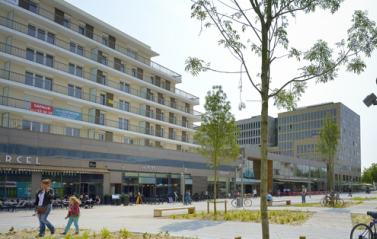
\includegraphics[width=0.55\linewidth]{outsiderivesdelorne}
\caption{The mall Rives de l'Orne.}
\label{fig:outsidemall}
\end{center}
\end{figure}

The test facilities concerns the mall ``Rives de l'Orne'' (see Fig. \ref{fig:outsidemall}). Rives de l'Orne\footnote{\url{http://www.rivesdelorne.com}} is a 
new and modern mall
situated in the city of Caen (France). It is composed of two face-to-face buildings separated by a large
main square (see Fig. \ref{fig:map}). At the first floor of the two buildings, there are many shops and restaurants. In the main square, there is a cinema. This space is surrounded by tramway stations and a train station.

\begin{figure}[!t]
\begin{center}
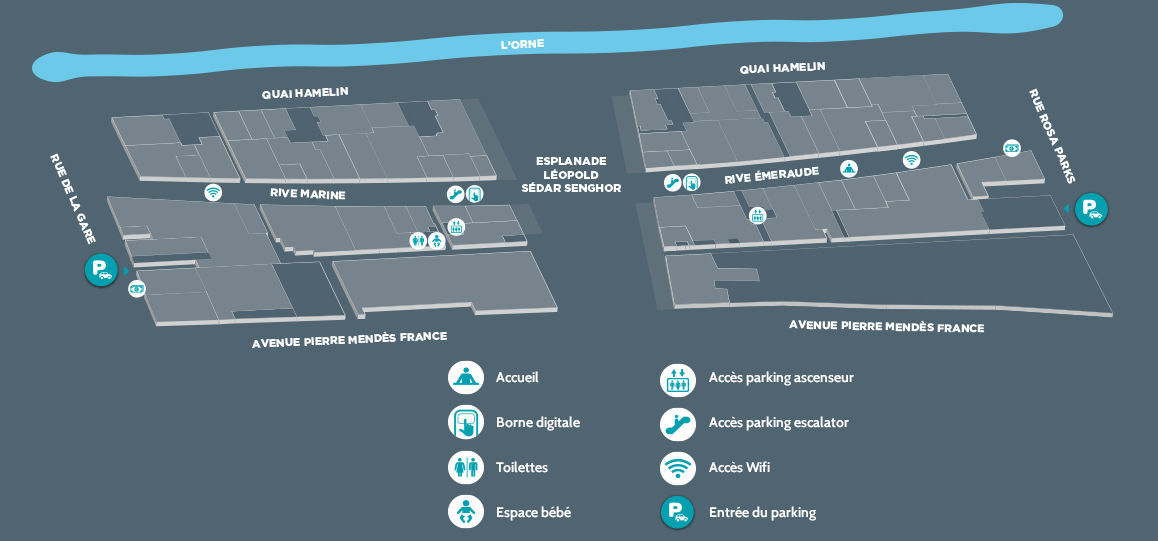
\includegraphics[width=1.0\linewidth]{mallplan}
\caption{The map of the mall.}
\label{fig:map}
\end{center}
\end{figure}

The mall is visited by more than 100,000 customers every year. In addition to customers,
several elderly people
live in the apartments located at the other floors of the buildings. These people have their habit and there are frequent customers of the mall (see Fig. \ref{fig:insidemall}).

\begin{figure}[!t]
\begin{center}
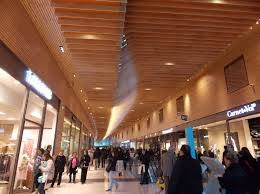
\includegraphics[width=0.5\linewidth]{InsideRivedelOrne}
\caption{Inside the mall Rives de l'Orne.}
\label{fig:insidemall}
\end{center}
\end{figure}

Two meetings have been organized ($23^{th}$ October 2014 and $12^{th}$ December 2014) to define the equipment to be installed, in terms of cameras and sensors.
Regarding the sensors, Radio-Frequency IDentification (RFID) tags and receivers will be used.
Cameras and sensors are in charge of sending information to the COACHES robots
about
\begin{itemize}
\item the shops;
\item the planning of the robot deployment in the mall;
\item the scheduled dissemination actions.
\end{itemize}

A visit of all COACHES project partners have been organized during the kickoff meeting,
held on $27^{th}$ and $28^{th}$ October 2014 in Caen. 


\section{Use cases for short-term interaction and navigation}

COACHES project envisages the implementation of a set of use cases
to show the feasibility of the approach and to assess the effectiveness
of the proposed solutions with actual users.
To this end, different use cases will be implemented, focusing on two main
components of the entire system:
\begin{enumerate}
\item Short-term human-robot interaction;
\item Safe navigation.
\end{enumerate}

Four use cases are described in the following. The use case are designed
to allow a short-term interaction between the COACHES robot and the human users.
In order to accomplish the required tasks, the robot must navigate
safely the environment. Navigation inside a populated environment, i.e., a mall
during opening hours, must be done in order to avoid damage to people
and goods.


\subsection{Customers ask for help carrying bags}

The robot is called by a shop manager (or by a customer) to help
in carrying bags. Bag loading operations take place in dedicated areas,
located at the exit of the shops.
The robot has to
\begin{enumerate}
\item Reach the exit of the shop;
\item Approach the dedicated bag loading area.
\end{enumerate}

\noindent When in position, the robot waits for the customer to establish
a contact.
Once the customer has established a contact, the robot asks the user
to load the bag in the bin carried by the robot.
Once the bag is loaded, the robot asks the customer if she/he is in a hurry.
If the customer is in a hurry, the robot
\begin{enumerate}
\item sets its speed to an high value;
\item proceeds to the mall parking lot.
\end{enumerate}

\noindent In the other case, the robot
\begin{enumerate}
\item sets its speed to a low value;
\item proceeds to the mall parking lot, proposing intermediate stops to shops
with interesting discounts.
\end{enumerate}


\subsection{Proposing an ice cream to a child}

The manager of an ice cream shop asks the robot to inform children about
a special discount. The robot looks around for children. When it detects
a child, the robot approaches her/him and it informs her/him
about the special discount. The child
is passionate about having an ice cream, but before guiding her/him
to the ice cream shop, the robot
\begin{enumerate}
\item asks for the parent's authorization.
\item waits for the positive parent's reply.
\end{enumerate}

\noindent Once the parent agrees to allow the child to follow the robot, it proceeds
to the ice cream shop. 


\subsection{Customer refuses the first robot proposal and accepts a different one}

The sales manager of a cinema inside the mall needs to promote a special discount
for a movie. The discount is loaded by the manager into the 
knowledge base (KB) of the robot, that contains the list of all the active commercial offers.
The robot is also aware, in his persistent KB, of the
existence of other secondary discounts.

Since there are no people moving around the robot, it starts
waiting for customers by monitoring the scene. As soon as the robot
sees a potential user (moving at the right distance and at the right speed),
the robot intercepts the customer and it asks her/him if she/he is interested
in the special discount for the movie.

The user answers that she/he is not interested.
Then, the robot asks the user to slide her/his personal customer card in order to
obtain a different available discount, in accordance to the user's previous purchases.

After the card data has been read, the robot finds out that the customer is a woman and that she
has made many purchases in the personal care department. 
Thus, the robot, by analysing the list of all the active commercial offers,
infers that the special discount about a facial cream could be of interest
to her.

Once informed of the discount, the customer reveals
that she is interested in it and she asks the robot for directions to reach the specific
shop. The robot safely guides the customer to the shop.


\subsection{Customer asks for directions in a crowded environment}

The robot has the objective to inform customers of available discounts.
The shopping mall is very crowded and, for safety
reasons, the robot decides that it should not move around, but
that is more convenient to wait
for users to approach it.

As soon as it detects a user, standing still at
the appropriate social distance and looking at her/him, the robot initiates
a conversation and it announces the available offers.

The user is interested in a listed offer
and she/he asks for directions to reach the shop offering a discount.
Since the robot cannot safely move due to the crowded environment, it
\begin{enumerate}
\item shows the user the desired path on its tablet;
\item informs the user that 20 meters away along the corridor she/he will find another robot,
that can provide more specific information, if needed.
\end{enumerate}

\noindent The human thanks the robot and proceeding to the next one in order to
receive further directions.
